
\textbf{Embedded gdagent{}}\\
\begin{itemize}
\item If you are starting your \gdaut{} and running your tests on your local machine, 
you can now connect to an embedded \gdagent{} directly from the \ite. 
\item This saves you having to start an \gdagent{} on localhost. 
\item This is also useful for testers working with \jb{} as a feature in an Eclipse installation. 
\item The embedded \gdagent{} is started on port 60000 by default; this number can be changed in the preferences.

\begin{figure}[h]
\begin{center}
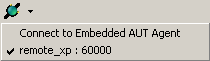
\includegraphics[width=0.60\textwidth]{52/ps/EmbeddedAgent}
\caption{Embedded AUT Agent}
\label{RNEmbeddedAgent}
\end{center}
\end{figure}


\end{itemize}


\textbf{Refactor: Replace with \gdcase{}}
\begin{itemize}
\item In the \gdtestcaseeditor{} and \gdtestsuiteeditor{}, there is a new option to replace one or more selected \gdcases{} with another \gdcase{} from the library. 
\item A new wizard takes you step-by-step through the replacement process, letting you transfer component names, match parameters and add further information for the new \gdcase{}.
\item This feature should help testers who want to restructure their tests after creating a reusable module to replace one or more \gdcases{}. 
\end{itemize}

\textbf{\gdomeditor{}: Cleanup unused component names}

\begin{itemize}
\item In the \gdomeditor{}, there is a new option in the context-sensitive menu. 
\item Via \bxmenu{Cleanup}{unused component names}{} \\
you can start a search for any component names that are no longer used in \gdsuites{} for this \gdaut{}. 
\item Once the search is finished, you can delete all of these unused names from the \gdomeditor{}. If they are then no longer used in the entire \gdproject{}, 
they can be deleted from the \gdcompnamebrowser{}. 

\begin{figure}[h]
\begin{center}
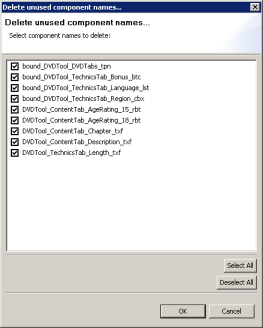
\includegraphics[width=0.60\textwidth]{52/ps/DeleteUnusedCompNames}
\caption{Deleting unused Component Names}
\label{RNDeleteUnusedCN}
\end{center}
\end{figure}
		
\end{itemize}

\textbf{HTML Test Result Reports can be expanded again}
\begin{itemize}
\item Following changes made for the initial contribution to Eclipse, the HTML Test Result Reports could not be viewed properly in the previous version. 
\item In this release, the nodes in the HTML reports can be expanded and collapsed to view the whole test progress. 

\begin{figure}[h]
\begin{center}
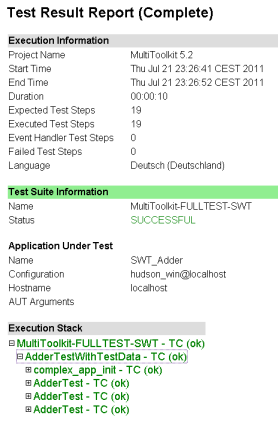
\includegraphics[width=0.60\textwidth]{52/ps/HTMLReport}
\caption{HTML Reports}
\label{RNHTMLReport}
\end{center}
\end{figure}
		
\end{itemize}

\textbf{State of component recognition displayed when collecting technical names}
\label{RNCompRec}
\begin{itemize}
\item When a component (technical name) is collected from an \gdaut{}, it receives a colored
dot corresponding to the accuracy of the object recognition for this component \textit{at the time of collecting}.
\begin{description}
\item [A green dot]{signifies that the component could be found with an exact match, and was the only component above the threshold}.
\item [A yellow dot]{means that the component is an exact match, but that multiple other components were also above the threshold.}
\item [A red dot]{ means that this component cannot be relocated in the current state of the \gdaut{}}
\end{description}
\item As a side effect, the colors on the component names (green) and technical names (red) that were displayed in previous versions are now no longer shown. Once the \gdomeditor{} has been saved, all names are shown with plain black icons. 
\begin{figure}[h]
\begin{center}
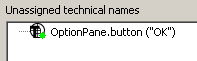
\includegraphics[width=0.6\textwidth]{52/ps/ColorDot}
\caption{Colored Dots for Object Mapping}
\label{RNColorDot}
\end{center}
\end{figure}
\end{itemize}

\textbf{Migration wizard re-enabled}
\begin{itemize}
\item  When migrating to the new version of \app{}, the migration assistant will automatically notify you that your database scheme is out-of-date. 
\item You can then select which \gdprojects{} to import (these must have been exported from the \gddb{} prior to migrating!).
\item The assistant will drop the tables in the \gddb{}, recreate the necessary tables and import the \gdprojects{} you specified.

\begin{figure}[h]
\begin{center}
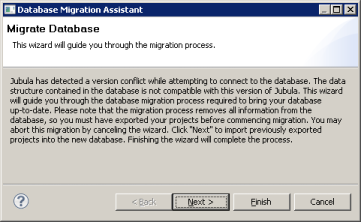
\includegraphics[width=0.6\textwidth]{52/ps/Migration}
\caption{Migration Wizard}
\label{RNMigration}
\end{center}
\end{figure}

\end{itemize}


\textbf{Copy ID to Clipboard also for \gdsuites{}}
\begin{itemize}
\item The ability to copy a unique ID to the clipboard to reference a \app{} element in external systems has also been implemented for \gdsuites{}. 
\item You can now copy the ID of a \gdcase{} or a \gdsuite{} to the clipboard, and also open an element based on its ID in the clipboard using \bxkey{Shift+F9}
\end{itemize}

\textbf{The DBTool is more verbose}
\begin{itemize}
\item The command line tool to import, export and delete \gdprojects{} in the \gddb{}, the DBTool, has been updated so that it is more verbose.
\end{itemize}

\textbf{Progress View}
\begin{itemize}
\item The \ite{} now  uses the progress view to show longer-running activities such as test execution, connecting to \gdauts{} etc.
\end{itemize}

\textbf{Edit Parameters Dialog in \gddataeditor{} can be opened via double-click}
\begin{itemize}
\item In the \gddataeditor{}  it is no longer necessary to open the Edit Parameters Dialog via context-menu, as it can now also be opened via double-click on the data set you wish to edit.
\end{itemize}


\textbf{Mac keyboards now supported, new mechanism for adding keyboard layout files}
\begin{itemize}
\item In the \gdaut{} configuration dialog for SWT and RCP \gdauts{}, the \bxname{Keyboard Layout} combo box now only offers 
layouts that have been defined for \app{}. German (DE) and English (US) are defined as standard. 
\item As well as being able to add keyboard layouts for other keyboards, you can also define platform-specific keyboard layouts (e.g. for Mac)
\item The documentation has been updated to describe the new mechanism for adding keyboard layouts.
\end{itemize}

\textbf{Object mapping: Degree of recognition accuracy for a test run can be viewed}
\begin{itemize}
\item The \gdomeditor{} has been extended so that the accuracy of component recognition is persisted and can be displayed.  
\item As well as displaying the state of component recognition when a technical name is collected from the \gdaut{} \bxpref{RNCompRec}, the degree of recognition accuracy is also noted 
for each test run. 
\item You can see the values for the recognition accuracy in two new BIRT reports in \app{}.
\begin{description}
\item [OMNameQuality]{shows a breakdown of the component names used in your test, and displays the degree of accuracy they were located during the test. You can use this report to see whether there are any component names that may need to be remapped (i.e. who are close to the threshold of not being found) before the test encounters a \bxname{Component Not Found} error. }
\item [OMNameQualityChart]{This report is a visual (graph) representation of the accuracy with which components were located during the test run. You can use the report to help you decide which components may need to be remapped, as they may soon result in a \bxname{Component Not Found} error during the test.}
\end{description}
\end{itemize}

\textbf{Mylyn: Refactored \gdcases{} are added to context}
\begin{itemize}
\item When working on a Mylyn task in app{}, \gdcases{} you create using the \bxname{refactor} function are now automatically added to the context.
\end{itemize}

\textbf{Mylyn: \gdcases{} opened via \bxkey{Ctrl+Shift+T} are added to context}
\begin{itemize}
\item When working on a Mylyn task in \app{}, \gdcases{} opened using the key combination \bxkey{Ctrl+Shift+T} are now automatically added to the context.
\end{itemize}

\textbf{Mylyn: \gdcases{} added via \gdcase{} reference dialog are added to context}
\begin{itemize}
\item When working on a Mylyn task in \app{}, \gdcases{} added using the \bxname{Add \gdcase{} reference} dialog are now automatically added to the context.
\end{itemize}

\textbf{Teststyle: Rules can now be viewed via the \gdpropview{}}
\begin{itemize}
\item When working with Teststyle, you can now open the \gdproject{} properties dialog to see the rule that has been flouted via:\\
\bxmenu{Show Teststyle Rule}{}{}\\
from the \gdprobview{}.
\end{itemize}

\textbf{Changes to BIRT reports}
\begin{itemize}
\item The BIRT report GUIdancerFULL has been removed.
\item There are new BIRT reports:
\begin{itemize}
\item \bxname{GUIdancerComments} shows a table of all failed relevant tests for the time specified, including the comment title that can be entered in the \gdtestsummaryview{}. This report is useful for delivering daily status reports of the tests.
\item \bxname{GUIdancerDuration} shows the duration of the chosen tests.
\item \bxname{GUIdancerExecutionHistogram} shows the proportion of executed, failed and non-executed \gdsteps{} for a test. This report is most useful when one specific \gdsuite{} is compared to see its progress over time. 
\item \bxname{TestresultSummary} shows a table of the \gdtestsummaryview{} for the dates and tests chosen. 
\end{itemize}
\item You can now also enter the \gdjob{} as a parameter for the report. The \gdsuites{} in the \gdjob{} are still displayed individually, however. 
\end{itemize}



\textbf{License Dialog: Restart prompt}
\begin{itemize}
\item Once a license has been added via the Preferences, a dialog is shown to remind you to restart \app{} before continuing. 
\item From the dialog you can choose to restart \app{} automatically.
\end{itemize}
